%----------------------------------------------------------------------------------------
%	PACKAGES AND THEMES
%----------------------------------------------------------------------------------------

\documentclass[aspectratio=169]{beamer}

\mode<presentation> {

  %%{ Themes

  % \usetheme{default}
  % \usetheme{AnnArbor}
  % \usetheme{Antibes}
  % \usetheme{Bergen}
  % \usetheme{Berkeley}
  % \usetheme{Berlin}
  \usetheme{Boadilla}
  % \usetheme{CambridgeUS}
  % \usetheme{Copenhagen}
  % \usetheme{Darmstadt}
  % \usetheme{Dresden}
  % \usetheme{Frankfurt}
  % \usetheme{Goettingen}
  % \usetheme{Hannover}
  % \usetheme{Ilmenau}
  % \usetheme{JuanLesPins}
  % \usetheme{Luebeck}
  % \usetheme{Madrid}
  % \usetheme{Malmoe}
  % \usetheme{Marburg}
  % \usetheme{Montpellier}
  % \usetheme{PaloAlto}
  % \usetheme{Pittsburgh}
  % \usetheme{Rochester}
  % \usetheme{Singapore}
  % \usetheme{Szeged}
  % \usetheme{Warsaw}

  %%}

  %%{ Color themes

  % \usecolortheme{albatross}
  % \usecolortheme{beaver}
  % \usecolortheme{beetle}
  % \usecolortheme{crane}
  % \usecolortheme{dolphin}
  % \usecolortheme{dove}
  % \usecolortheme{fly}
  % \usecolortheme{lily}
  % \usecolortheme{orchid}
  % \usecolortheme{rose}
  % \usecolortheme{seagull}
  \usecolortheme{seahorse}
  % \usecolortheme{whale}
  % \usecolortheme{wolverine}

  %%}

  %!TEX root = main.tex

\definecolor{CVUTBLUE}{RGB}{0,121,194}
\definecolor{CVUTBLUEDECREASED}{RGB}{0,141,204}
\definecolor{CVUTBLUEDECREASED2}{HTML}{bfcfe4}

\setbeamercolor{frametitle}{fg=white,bg=CVUTBLUE}

\setbeamertemplate{itemize items}[circle]
\setbeamercolor{itemize item}{fg=CVUTBLUE}

\setbeamercolor{section in head/foot}{bg=CVUTBLUE!0!black,fg=CVUTBLUE}
\setbeamercolor{institute in head/foot}{fg=CVUTBLUE}

\setbeamercolor*{palette primary}{fg=white,bg=CVUTBLUE}
\setbeamercolor*{palette secondary}{fg=white,bg=CVUTBLUEDECREASED}
\setbeamercolor*{palette tertiary}{fg=white,bg=CVUTBLUE}
\setbeamercolor*{palette quaternary}{fg=white,bg=black}
\setbeamercolor*{palette quinary}{fg=white,bg=CVUTBLUE}
\setbeamercolor*{palette senary}{fg=CUBlue,bg=white}

\setbeamercolor{title}{fg=white,bg=CVUTBLUE}

\setbeamercolor{block title}{fg=black,bg=CVUTBLUEDECREASED2}
\setbeamercolor{block body}{fg=black,bg=white}

%\definecolor{cblue}{RGB}{0,121,194}
%\def\blb{\color{cblue}\bf }

\setbeamertemplate{frametitle}
{
    \nointerlineskip
    \begin{beamercolorbox}[sep=0.0cm,ht=1.3em,wd=\paperwidth]{frametitle}%
        \vbox{}\vskip0.2ex%
        \hspace*{0.2em}\strut\insertframetitle\strut
        \hfill
        \raisebox{-0.4ex}{
\includegraphics[width=3cm]{fig/logo_ctu_fee_mrs_white.png}}\hspace*{0.3ex}
        \vskip-0.2ex%
    \end{beamercolorbox}
}


  % \setbeamertemplate{footline} % remove the footer line
  % \setbeamertemplate{footline}[page number] % replace the footer line with simple numbers

  \setbeamertemplate{navigation symbols}{}
  \setbeamertemplate{bibliography item}{\insertbiblabel} % removing the navigation symbols

  % \setbeamerfont{bibliography item}{size=\tiny}
  % \setbeamerfont{bibliography entry author}{size=\tiny}
  % \setbeamerfont{bibliography entry title}{size=\tiny}
  % \setbeamerfont{bibliography entry location}{size=\tiny}
  % \setbeamerfont{bibliography entry note}{size=\tiny}

}

%%{ Docu HEAD

\usepackage{graphicx} % Allows including images
\usepackage{booktabs} % Allows the use of \toprule, \midrule and \bottomrule in tables
\usepackage{multimedia}
\newcommand{\superfill}{\vskip0pt plus 1filll}

\usepackage{isotope}
\usepackage{animate}

\usepackage[export]{adjustbox}

\usepackage{graphicx}
\usepackage{setspace}
\usepackage{epstopdf}
\usepackage{float}
\usepackage{multirow,tabularx,makecell}

\usepackage{amsmath,amsfonts,amssymb,bm}

\usepackage[backend=bibtex,defernumbers=true,style=ieee,sorting=none,sortcites=false]{biblatex}

\renewcommand*{\bibfont}{\normalfont\tiny}

% Print labelnumbers with suffixes, adjust secondary labelnumber 2/2
\DeclareFieldFormat{labelnumber}{%
  \ifkeyword{mine}
    {\ifkeyword{core}
      {{\number\numexpr#1}c}%
      {{\number\numexpr#1}a}%
    }%
    {#1}%
}

\DeclareCiteCommand{\tabcite}%[\mkbibbrackets]
  {\usebibmacro{cite:init}%
   \usebibmacro{prenote}}
  {\usebibmacro{citeindex}%
   \usebibmacro{cite:comp}}
  {}
  {\usebibmacro{cite:dump}%
   \usebibmacro{postnote}}

% {{\number\numexpr#1-\value{bbx:primcount}}a}

%%{ fullcite box

\usepackage{tcolorbox}

\definecolor{light-gray}{gray}{0.95}
\newcommand{\fullciteinbox}[2]{%

\DeclareCiteCommand{\fullcite}
{\usebibmacro{prenote}}
{\clearfield{addendum}%
  \usedriver
  {\defcounter{minnames}{6}%
  \defcounter{maxnames}{6}}
{\thefield{entrytype}}}
{\multicitedelim}
{\usebibmacro{postnote}}

%\vspace{3em}%
%\raisebox{3em}[3em][3em]{%
% \vspace{-0.2em}
\begin{tcolorbox}[width=\textwidth,colback={light-gray},title={}]%
\begin{minipage}[t]{0.07\linewidth}%
\raggedright%
\scriptsize \cite{#1}%
\end{minipage}%
\begin{minipage}[t]{0.93\linewidth}%
\scriptsize \fullcite{#1}%
\ifx&#2&
\else
  \\
  \url{#2}
\fi
\end{minipage}%
\end{tcolorbox}%
%}%
\vspace{-0.3em}
}%

%%}

\addbibresource{main.bib}

\defbibenvironment{favoritebib}
{\itemize}
{\enditemize}
{\item}
\usepackage{siunitx}
\DeclareSIUnit \parsec {pc}
\DeclareSIUnit \electronvolt {eV}
\DeclareSIUnit \pixel {px}
\DeclareSIUnit \arcmin {arcmin}
\DeclareSIUnit \erg {erg}
\DeclareSIUnit \joul {J}

\usepackage{enumitem} % To enable enumerate with letters (a, b, c...)
\newlist{alphalist}{enumerate}{1}
\setlist[alphalist]{label=\alph*)}
\setlist[itemize]{label=\textbullet}

\usepackage{cellspace}
\newcolumntype{D}{>{\hfill}N{3}{2}<{\hfill}}
\newcommand*\cellspacelimit[2]{\setlength{\cellspacetoplimit}{#1}\setlength{\cellspacebottomlimit}{#2}}

% figures
\usepackage{wrapfig}
% \usepackage[font={footnotesize}]{caption}
\usepackage[font={small}]{caption}
% \usepackage{subcaption}

% subfloat
\usepackage{subfig}
% \usepackage[export]{adjustbox}

\usepackage{color}
\usepackage{url}

%%{ tikz

\usepackage{tikz}
\usepackage{pgfplots}
\pgfplotsset{compat=1.14}
\usetikzlibrary{backgrounds,arrows,automata,shapes,positioning,calc,through,spy,shapes,shapes.geometric,shapes.multipart,fit,patterns,fadings}
\pgfdeclarelayer{background}
\pgfdeclarelayer{foreground}
\pgfsetlayers{background,main,foreground}

\tikzset{
  state/.style={
    rectangle,
    draw=black, very thick,
    minimum height=1.0em,
    text centered,
  },
  state_red/.style={
    rectangle,
    draw=black, very thick,
    minimum height=1.0em,
    text centered,
    fill=red,
  },
  state_focus/.style={
    rectangle,
    draw=black, very thick,
    minimum height=1.0em,
    text centered,
    fill=black!50,
  },
  smallstate/.style={
    rectangle,
    draw=black, very thick,
    minimum height=0.2em,
    text centered,
  },
  final_state/.style={
    rectangle,
    rounded corners,
    draw=black, very thick,
    minimum height=2em,
    text centered,
  },
  initial_state/.style={
    rectangle,
    double=white,
    double distance=1pt,
    inner sep=2pt,
    draw=black, very thick,
    minimum height=2em,
    text centered,
  },
  point/.style={
    circle,
    inner sep=0pt,
    minimum size=3pt,
    fill=red
  },
  adder/.style={
    circle,
    inner sep=2pt,
    minimum size=0.3in,
    draw=black, very thick,
    text centered
  },
  state_gray/.style={
    rectangle,
    draw=black, very thick,
    fill=gray!40,
    minimum height=1.0em,
    text centered,
    inner sep=0,
  },
  state_white/.style={
    rectangle,
    draw=black, very thick,
    fill=white,
    minimum height=1.0em,
    text centered,
    text=black,
    inner sep=0,
  },
  state_blue/.style={
    rectangle,
    draw=black, very thick,
    fill=blue!40,
    minimum height=1.0em,
    text centered,
    text=black,
    inner sep=0,
  },
  final_state/.style={
    rectangle,
    rounded corners,
    draw=black, very thick,
    minimum height=2em,
    text centered,
  },
  initial_state/.style={
    rectangle,
    double=white,
    double distance=1pt,
    inner sep=2pt,
    draw=black, very thick,
    minimum height=2em,
    text centered,
  },
  point/.style={
    circle,
    inner sep=0pt,
    minimum size=3pt,
    fill=red
  },
}


\tikzset{
    imgletter/.style={
      rectangle,
      inner sep=2pt,
      rounded corners=.1em,
      text=black,
      minimum height=1em,
      text centered,
      fill=white,
      fill opacity=1.0,
      text opacity=1,
      anchor=south west,
  },
}

%%}

\usepackage{pdfpc-movie}
\newcommand{\mymovie}[3][]{\pdfpcmovie[#1]{#2}{#3}}
% \newcommand{\mymovie}[3][]{\movie[#1]{#2}{#3}}

%%{ ARROWS IN TIKZ

\tikzset{
  myarrow/.style={
    draw,
    fill=orange,
    single arrow,
    minimum height=3.5ex,
    single arrow head extend=1ex
  }
}

\newcommand{\arrowup}{%
  \vspace{-0.8em}
  \tikz [baseline=-0.5ex]{\node [myarrow,rotate=90] {};}
  \vspace{-1.4em}
}

\newcommand{\arrowdown}{%
  \vspace{-0.8em}
  \tikz [baseline=-1ex]{\node [myarrow,rotate=-90] {};}
  \vspace{-1.5em}
}

\newcommand{\arrowright}{%
  \tikz [baseline=-1ex]{\node [myarrow,rotate=0] {};}
}

\newcommand{\arrowleft}{%
  \tikz [baseline=-1ex]{\node [myarrow,rotate=180] {};}
}

%%}

%%{ CHECKMARK IN TIKZ

\def\checkmark{\tikz\fill[scale=0.4](0,.35) -- (.25,0) -- (1,.7) -- (.25,.15) -- cycle;}

%%}

\newcommand{\strong}[1]{\textbf{#1}}
\newcommand{\coord}[1]{\textbf{#1}}
\newcommand{\norm}[1]{\left\lvert#1\right\rvert}
\newcommand{\m}[1]{\ensuremath{\mathbf{#1}}}
\newcommand\numberthis{\addtocounter{equation}{1}\tag{\theequation}}
\newcommand{\corrected}[1]{{\color{black} {#1}}}
% \newcommand{\comment}[1]{{\color{blue} {#1}}}
\newcommand{\add}[1]{{\color{green} {#1}}}
\newcommand{\todo}[1]{{\color{red} TODO {#1}}}
\newcommand{\updated}[1]{{\color{blue} {#1}}}
\newcommand{\reffig}[1]{Fig.~\ref{#1}}
\newcommand{\refalg}[1]{Alg.~\ref{#1}}
\newcommand{\refsec}[1]{Sec.~\ref{#1}}
\newcommand{\reftab}[1]{Table~\ref{#1}}
\newcommand{\real}{\mathbb{R}}
\newcommand{\red}[1]{{\color{red} #1}}
\newcommand{\minus}{\scalebox{0.75}[1.0]{$-$}}
\newcommand{\plus}{\scalebox{0.8}[0.8]{$+$}}
\newcommand{\figvspace}{\vspace{-1em}} % this may eventually do something, so far just a placeholder

% \usepackage{pgf}
% \logo{\pgfputat{\pgfxy(0,5)}{\pgfbox[right,base]{\includegraphics[height=0.8cm]{}}}}
% \newcommand{\nologo}{\setbeamertemplate{logo}{}}

% \usepackage{eso-pic}
% \newcommand\AtPagemyUpperLeft[1]{\AtPageLowerLeft{\put(\LenToUnit{0.66\paperwidth},\LenToUnit{0.904\paperheight}){#1}}}
% \AddToShipoutPictureFG{
%   \AtPagemyUpperLeft{{
\includegraphics[height=0.85cm,keepaspectratio]{fig/logo_ctu_fee_mrs_blue.png}}}
% }
% \newcommand{\AddToShipoutPictureFG}{\setbeamertemplate{logo}{}}

%%}

%%{ TITLE PAGE


\title[Cooperative Sensing by a Group of UAVs]{Cooperative Sensing by a Group of Unmanned Aerial Vehicles}
\subtitle{Doctoral Thesis}
\author[Tomas Baca]{{Ing. Tomas Baca} \\
{\and} \\
{Supervisor: Ing. Martin Saska, Dr. rer. nat.} \\
{Supervisor-Specialist: Ing. Michal Platkevic, Ph.D.} \\
{\and} \\
{Ph.D. programme: Electrical Engineering and Information Technology} \\
{Branch of study: Artificial Intelligence and Biocybernetics}}

\institute[CTU in Prague] {
  \begin{small}
  Multi-Robot Systems group, Faculty of Electrical Engineering\\
  Czech Technical University in Prague
  \end{small}}

\date[September 26th, 2017]{}

\titlegraphic{
\includegraphics[width=5cm]{fig/logo_ctu_fee_mrs_blue.png}}

\begin{document}

\begin{frame}

  \titlepage % Print the title page as the first slide

\vphantom{\cite{stibinger2020localization}
          \cite{spurny2019cooperative}
          \cite{baca2019autonomous}
          \cite{baca2018timepix}
          \cite{baca2019timepix}
          \cite{baca2018model}
          \cite{baca2020autonomous}
          \cite{baca2021mrs}}%
\vphantom{\cite{petracek2020bioinspired}
          \cite{petrlik2020robust}
          \cite{saikin2020wildfire}
          \cite{saska2020formation}
          \cite{giernacki2019realtime}
          \cite{loianno2018localization}
          \cite{baca2018rospix}
          \cite{saska2017system}
          \cite{chudoba2016exploration}}%
\vphantom{\cite{roucek2019darpa}
          \cite{faigl2017onsolution}
          \cite{saska2017documentation}
          \cite{baca2017autonomous}
          \cite{saska2016formations}
          \cite{spurny2016complex}
          \cite{baca2016embedded}}%
\vphantom{\cite{roucek2021system}
          \cite{walter2021extinguishing}
          \cite{ahmad2021autonomous}
          \cite{dmytruk2021safe}
          \cite{kratky2021autonomous2}
          \cite{silano2021powerline}
          \cite{smrcka2021admittance}
          \cite{spurny2021autonomous}
          \cite{stasinchuk2021multiuav}
          \cite{baca2021gamma}
          \cite{vrba2020autonomous}
          \cite{walter2020extinguishing}}%
\vphantom{\cite{daniel2019inorbit}
          \cite{urban2017vzlusat}
          \cite{baca2016miniaturized}}%
\vphantom{\cite{daniel2017xray}
          \cite{daniel2016terrestrial}}%
\vphantom{\cite{urban2021rex}}%
\vphantom{\cite{chudoba2014localization}
          \cite{saska2013adhoc}}%
\vphantom{\cite{horla2021altune}
          \cite{horyna2021autonomous}
          \cite{petracek2021large}}%


\end{frame}

% \nologo

%%}

\section{Introduction}

\begin{frame}
  \frametitle{Outline}
  \tableofcontents
\end{frame}

\begin{frame}
  \frametitle{Outline}
  \tableofcontents[currentsection]
\end{frame}

\subsection{Research streams}

%%{ Research streams

\begin{frame}
\frametitle{Research streams}

\begin{columns}[c]

\column{0.31\textwidth}

\begin{block}{UAV systems}
  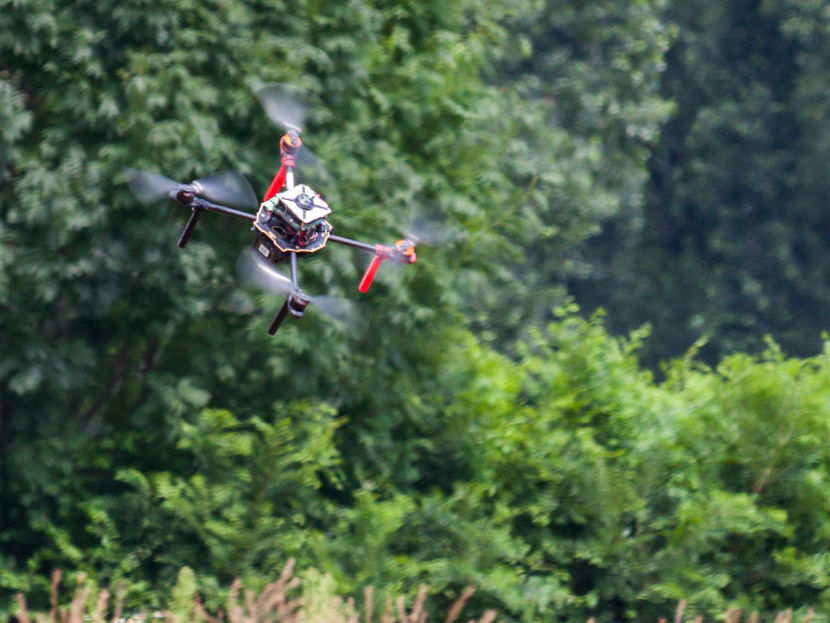
\includegraphics[width=1.0\textwidth]{./fig/drona.jpg}
  \begin{itemize}
    \item UAV control
    \item State estimation
    \item Trajectory tracking
    \item UAV deployment
  \end{itemize}
\end{block}

\column{0.31\textwidth}

\begin{block}{Remote sensing by UAVs}
  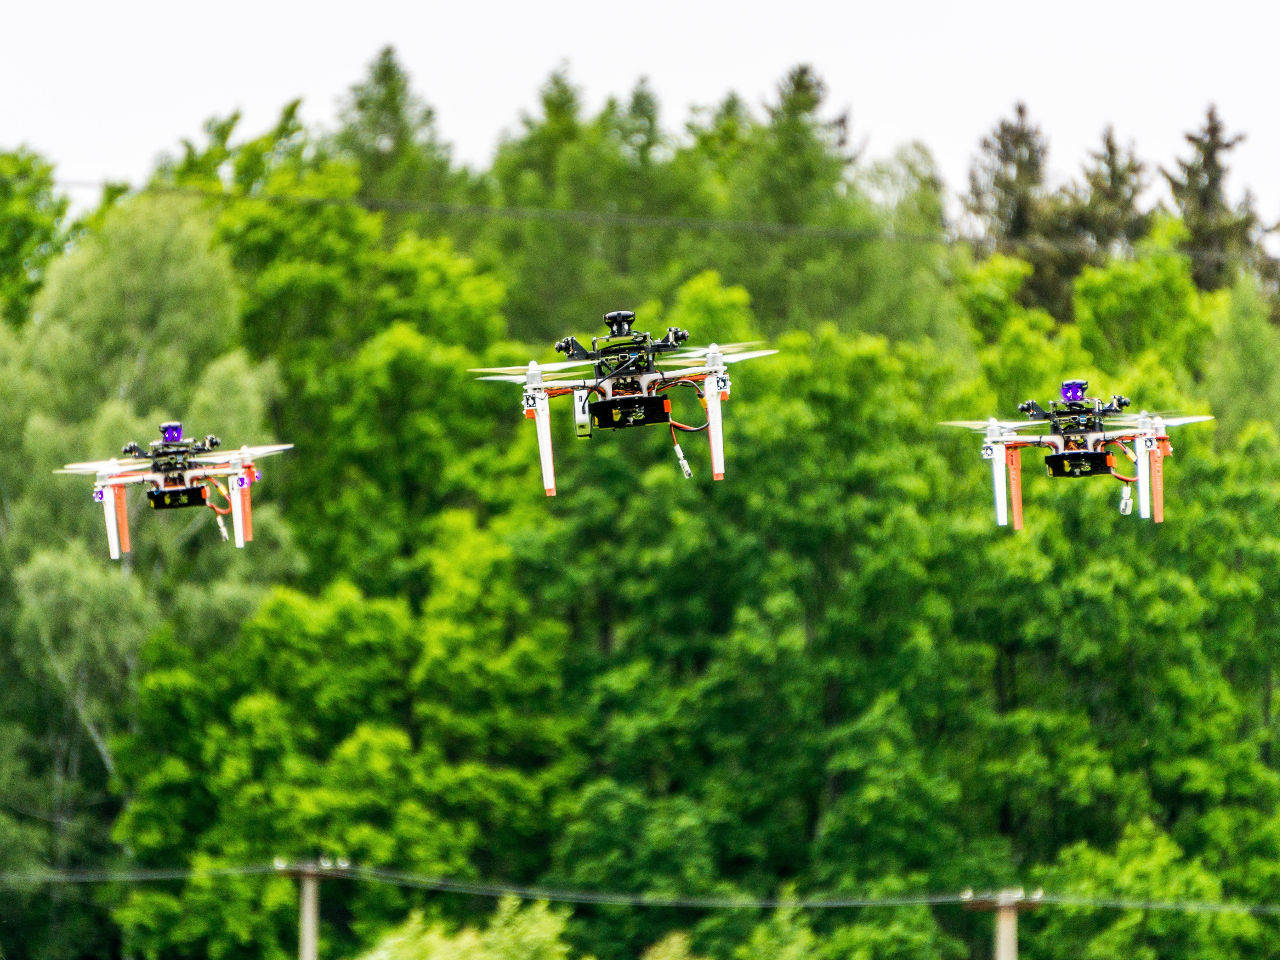
\includegraphics[width=1.0\textwidth]{./fig/photos/swarm_2_1-5.jpg}
  \begin{itemize}
    \item Object estimation
    \item Object manipulation
    \item Precise landing
    \item Swarming and flocking
  \end{itemize}
\end{block}

\column{0.31\textwidth}

\begin{block}{Radiation dosimetry}
  \begin{center}
    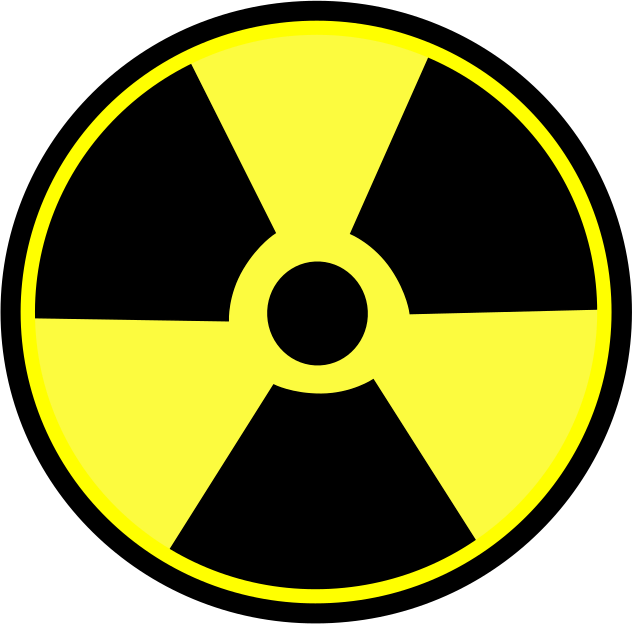
\includegraphics[width=0.70\textwidth]{./fig/photos/radioactive_sign.png}
  \end{center}
  \begin{itemize}
    \item Pixel detectors
    \item Space dosimetry
    \item Terrestrial dosimetry
    \item UAV Compton camera
  \end{itemize}
\end{block}

\end{columns}

\end{frame}

%%}

\section{Research stream 1: Multirotor-UAV system for research and real-world deployment}

\begin{frame}
  \frametitle{Outline}
  \tableofcontents[currentsection]
\end{frame}

%%{ Multirotor UAV system for research

\begin{frame}
\frametitle{Multirotor UAV system for research}

  \begin{block}{Motivation (2013 -- 2016)}
  \begin{itemize}
    \item research validation in real-world experiments \cite{spurny2016complex, saska2016formations, chudoba2016exploration, saska2017system, saska2017documentation, saska2013adhoc, chudoba2014localization}
    \item experimenting outside of laboratory conditions (desired)
  \end{itemize}
\end{block}

\begin{columns}[c]

\column{0.385\textwidth} % Left column and width

\begin{block}{Embedded MPC \cite{baca2016embedded}}
  \centering
  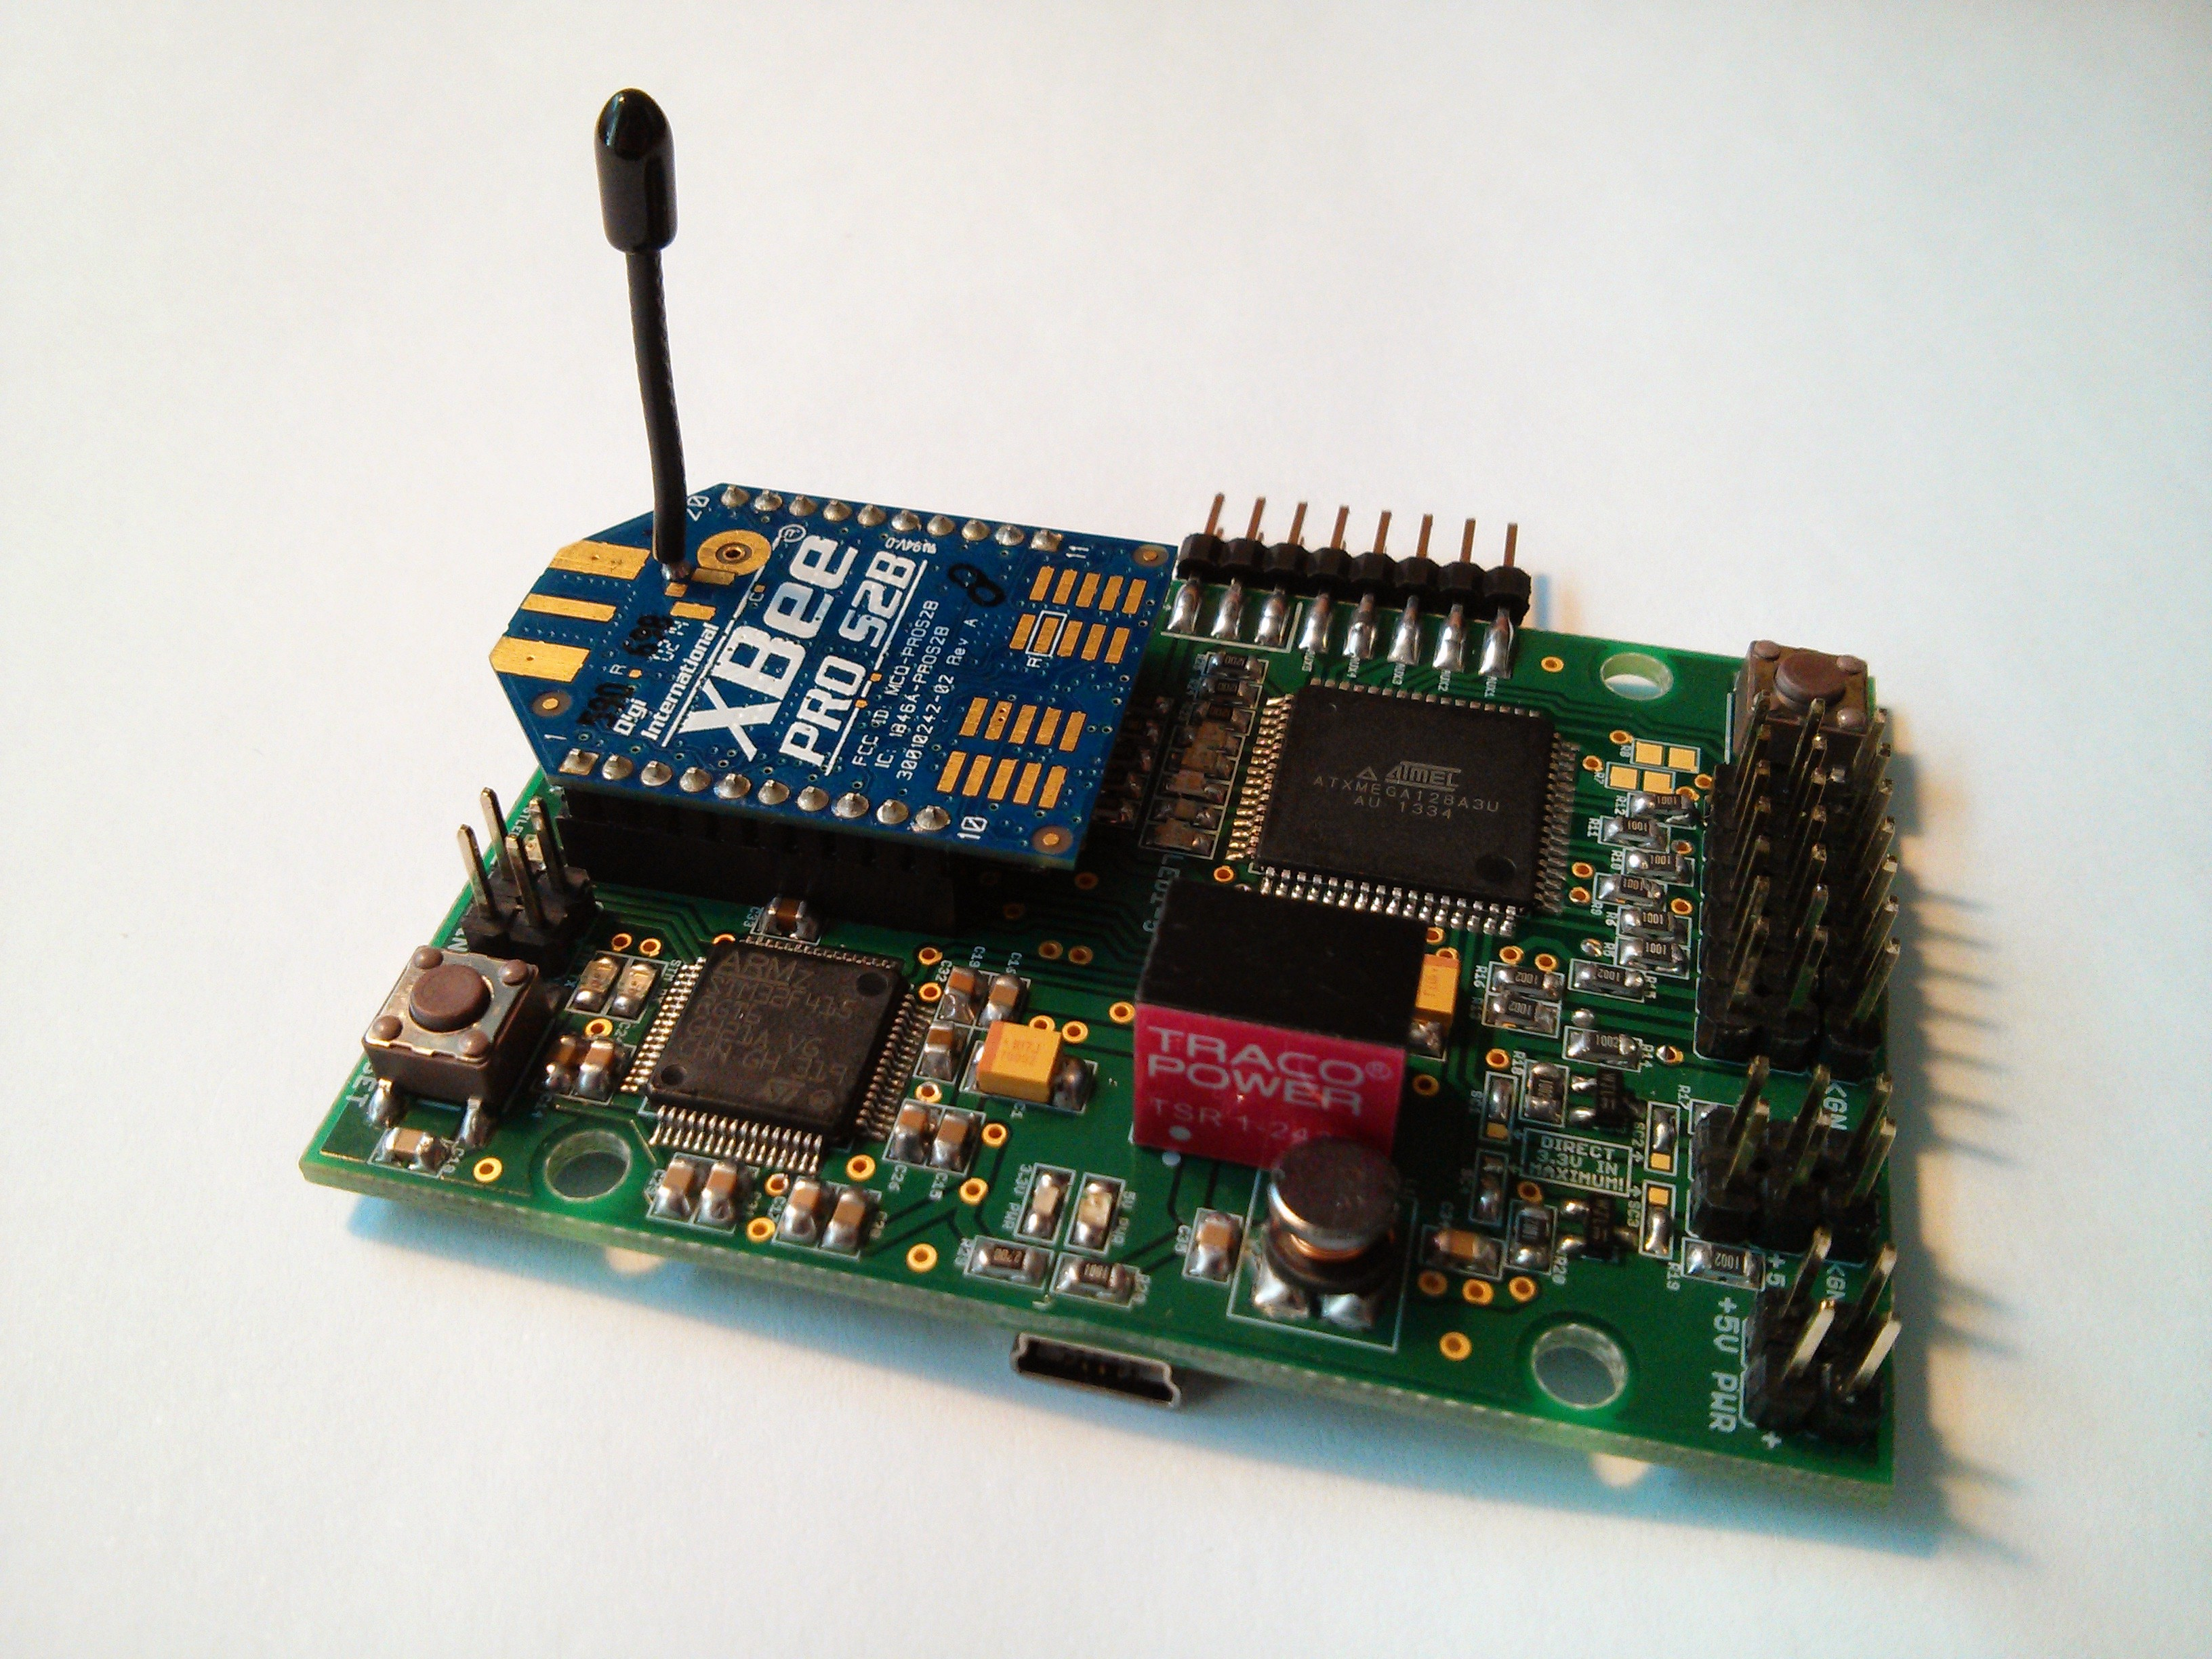
\includegraphics[width=1.0\textwidth]{./fig/photos/multirotor_control_board.jpg}
\end{block}

\column{0.57\textwidth} % Right column and width

\begin{block}{Multi-UAV formations \cite{spurny2016complex}}
  \centering
  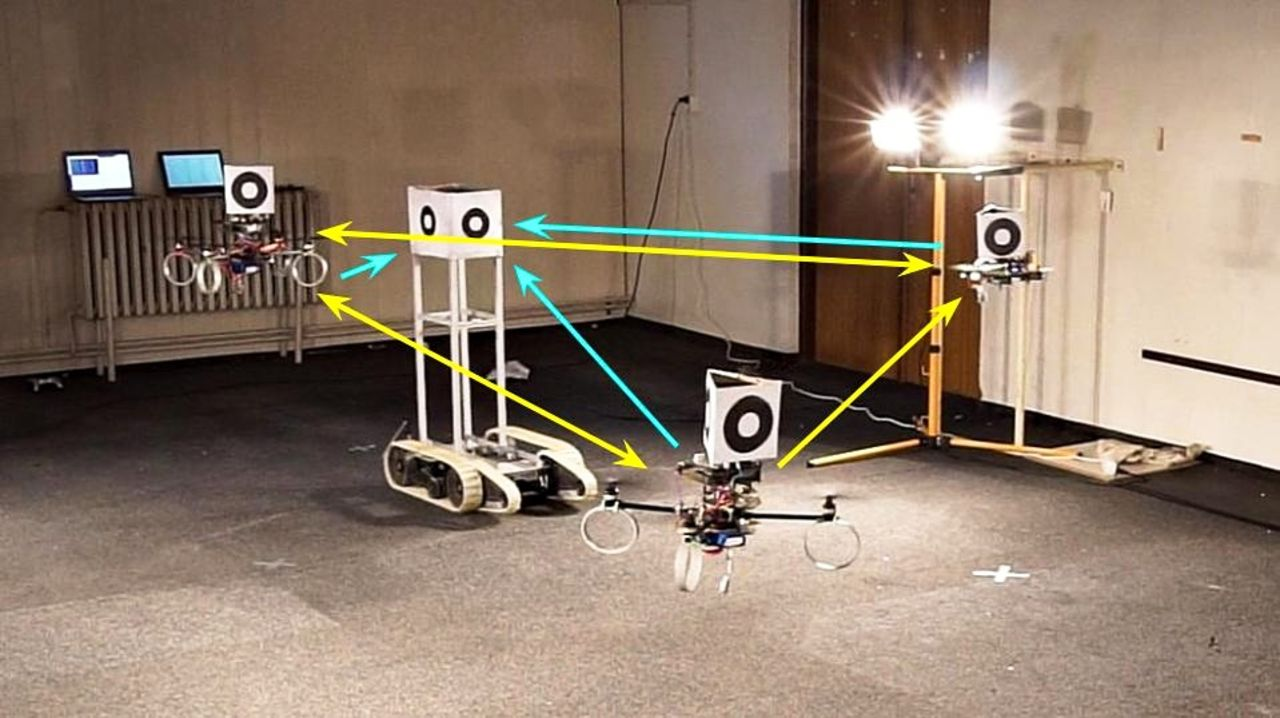
\includegraphics[width=0.9\textwidth]{./fig/photos/mav_rfid.jpg}
\end{block}

\end{columns}

\end{frame}

%%{ MPC Tracker

\begin{frame}
\frametitle{Model Predictive Control Tracker}

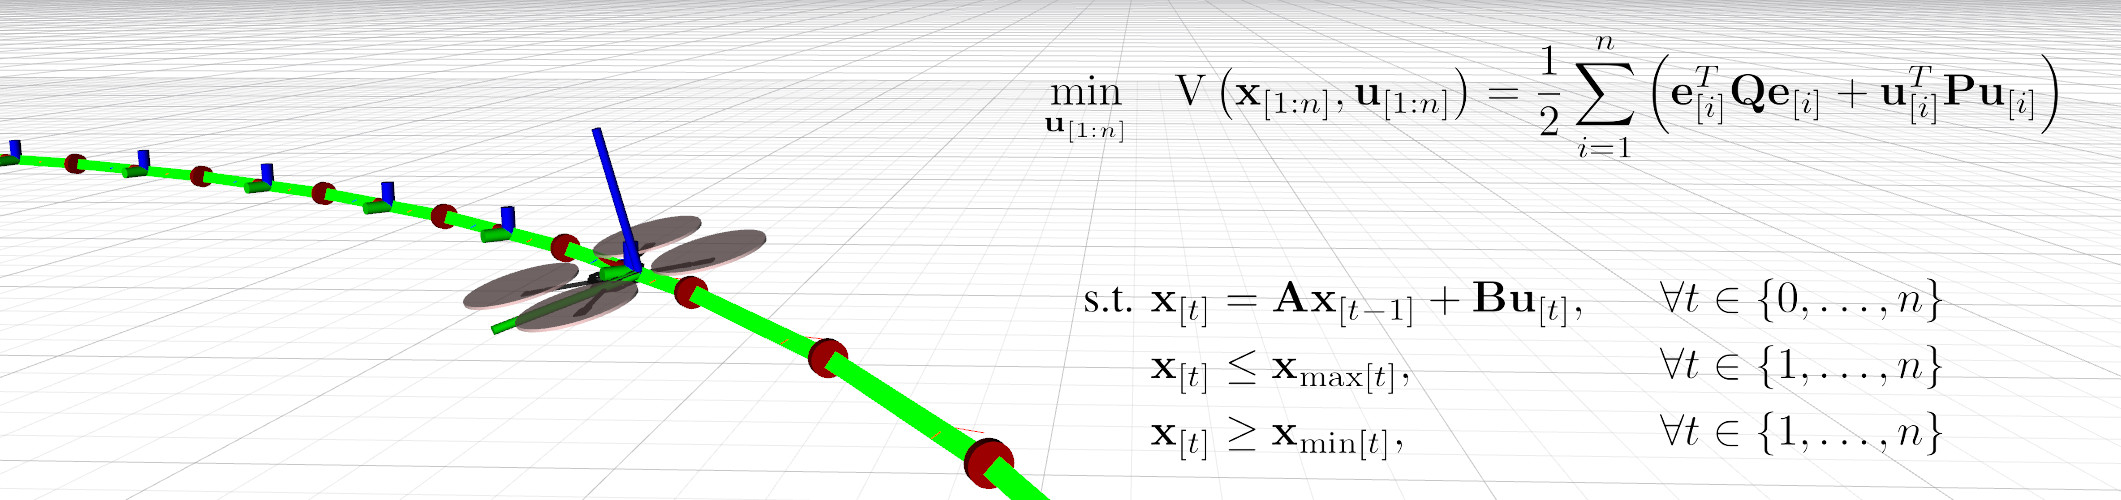
\includegraphics[width=1.0\textwidth]{./fig/photos/tracker.jpg}

% \fullciteinbox{baca2018model}{http://github.com/ctu-mrs/mrs_uav_trackers}
\fullciteinbox{baca2018model}{}

\end{frame}

\begin{frame}
\frametitle{Model Predictive Control Tracker}

\begin{columns}[c]

\column{0.48\textwidth} % Left column and width

\begin{block}{Problem}
  \begin{itemize}
    \item real-time reference generation
    \item \SI{100}{Hz} full state reference for controllers
    \item dynamic constraints satisfaction 
    \item user input: trajectory of poses
  \end{itemize}
\end{block}

\column{0.48\textwidth} % Right column and width

\begin{block}{Solution}
  
\end{block}

\end{columns}

\fullciteinbox{baca2018model}{}

\end{frame}

%%}

\begin{frame}
\frametitle{The MRS UAV System}

  \begin{block}{Block title}
    \begin{figure}
      \begin{adjustbox}{max totalsize={1.0\textwidth}{.65\textheight}, center}
        \pgfdeclarelayer{foreground}
\pgfsetlayers{background,main,foreground}

\tikzset{radiation/.style={{decorate,decoration={expanding waves,angle=90,segment length=4pt}}}}

\begin{tikzpicture}[->,>=stealth', node distance=3.0cm]

  \node[state, shift = {(0.0, 0.0)}] (user_software) {
      \begin{tabular}{c}
        \small Mission \\
        \small planner
      \end{tabular}
    };

  \node[state, right of = user_software, shift = {(0.6, 0.0)}] (collision_avoidance) {
      \begin{tabular}{c}
        \small Collision \\
        \small avoidance
      \end{tabular}
    };

  \node[state, right of = collision_avoidance, shift = {(0, -0)}] (mpc_tracker) {
      \begin{tabular}{c}
        \small MPC \\
        \small tracker
      \end{tabular}
    };

  \node[state, right of = mpc_tracker, shift = {(0, -0)}] (so3_controller) {
      \begin{tabular}{c}
        \small SO(3) \\
        \small controller
      \end{tabular}
    };

  \node[state, right of = so3_controller, shift = {(0.2, -0)}] (pixhawk) {
      \begin{tabular}{c}
        \small Attitude \\
        \small controller
      \end{tabular}
    };

  \node[state, right of = pixhawk, shift = {(0, -0)}] (uav_plant) {
      \begin{tabular}{c}
        \small UAV \\
        \small plant
      \end{tabular}
    };

  \node[state, below of = so3_controller, shift = {(0, 0.5)}] (state_observer) {
      \begin{tabular}{c}
        \small State \\
        \small observer
      \end{tabular}
    };

    \path[->] ($(user_software.east) + (0.0, 0)$) edge [] node[above, midway, shift = {(0.0, 0.05)}] {  
      \begin{tabular}{c}
        \small desired trajectory\\
        \small $\mathbf{r}_D, \phi_D$\\
        \small \textit{on demand}
    \end{tabular}} ($(collision_avoidance.west) + (0.0, 0.00)$);

    \path[->] ($(collision_avoidance.east) + (0.0, 0)$) edge [] node[above, midway, shift = {(0.0, 0.05)}] {  
      \begin{tabular}{c}
        \small reshaped trajectory\\
        \small $\mathbf{r}_R, \phi_R$\\
        \small \textit{100 Hz}
    \end{tabular}} ($(mpc_tracker.west) + (0.0, 0.00)$);

    \path[->] ($(mpc_tracker.east) + (0.0, 0)$) edge [] node[above, midway, shift = {(0.0, 0.05)}] {  
      \begin{tabular}{c}
        % \small $\textbf{x}_D, \dot{\textbf{x}}_D, \ddot{\textbf{x}}_D$ \\
        % \small $\phi_{D}, \dot{\phi}_D, \ddot{\phi}_D$\\
        $\textbf{x}_D$\\
        \small \textit{100 Hz}
    \end{tabular}} ($(so3_controller.west) + (0.0, 0.00)$);

    \path[->] ($(so3_controller.east) + (0.0, 0)$) edge [] node[above, midway, shift = {(0.0, 0.05)}] {  
      \begin{tabular}{c}
        \small $\textbf{R}\left(\phi_D, \theta_D, \psi_D\right)$ \\
        \small $T_D$ \\
        \small \textit{100 Hz}
    \end{tabular}} ($(pixhawk.west) + (0.0, 0.00)$);

    \path[->] ($(pixhawk.east) + (0.0, 0)$) edge [] node[above, midway, shift = {(0.0, 0.05)}] {  
      \begin{tabular}{c}
        \small motor \\
        \small control \\
        \small \textit{$\approx1$ kHz}
    \end{tabular}} ($(uav_plant.west) + (0.0, 0.00)$);

    \pgfmathsetmacro{\offsetA}{-1.5}
    \coordinate (under_mpc) at ($(mpc_tracker.south) + (0.0, \offsetA)$);
    \coordinate (under_avoidance) at ($(collision_avoidance.south) + (0.0, \offsetA)$);
    \path[-] ($(mpc_tracker.south) + (0.0, 0)$) edge [] (under_mpc) -- (under_mpc) edge [] (under_avoidance) edge [] node[above, midway, shift = {(0.0, 0.0)}] {  
      \begin{tabular}{c}
        \small predicted \\
        \small trajectory \\
        \small \textit{2 Hz}
    \end{tabular}} (under_avoidance) -- (under_avoidance) edge [->] ($(collision_avoidance.south) + (0.0, 0.0)$);
    \pgfmathsetmacro{\offsetB}{-0.45}
    \path[->] ($(collision_avoidance.south)+(+\offsetB, -3.5)$) edge [dashed] node[left, near start, shift = {(0.2, -0.3)}] {  
      \begin{tabular}{c}
        \small \corrected {predicted} \\
        \small \corrected {trajectory} \\
        \small \corrected {of other UAVs} \\
        \small \corrected {\textit{2 Hz}}
    \end{tabular}} ($(collision_avoidance.south)+(+\offsetB, 0)$);

    \draw[-, radiation, decoration={angle=45}] ($(collision_avoidance.south) + (\offsetB+0.14, -3.2)$) -- +(0:0.5);

    \pgfmathsetmacro{\offsetC}{0.0}
    \path[<-] ($(mpc_tracker.south)+(+\offsetC, -3.5)$) edge [dashed] node[left, near start, shift = {(0.2, -0.3)}] {  
      \begin{tabular}{c}
        \small predicted \\ 
        \small trajectory \\
        \small \textit{2 Hz}
    \end{tabular}} ($(mpc_tracker.south)+(+\offsetC, 0)$);

    \draw[-, radiation, decoration={angle=45}] ($(mpc_tracker.south) + (0.15, -3.2)$) -- +(0:0.5);
    % \draw[-, radiation, decoration={angle=45}] ($(mpc_tracker.south) + (+0.50, -3.5)$) -- +(90:0.5);

    \path[-] ($(state_observer.west)+(0, 0)$) edge [dotted] node[above, near end, shift = {(-1.2, 0.0)}] {  
      \begin{tabular}{c}
        \small UAV state \\
        \small estimate \\
        \small \textit{100 Hz}
    \end{tabular}} ($(user_software.south |- state_observer.west)$) -- ($(user_software.south |- state_observer.west)$) edge [->,dotted] ($(user_software.south)+(0, 0)$);

    \path[->] ($(state_observer.north)+(0, 0)$) edge [dotted] ($(so3_controller.south)$);

    \path[-] ($(pixhawk.south)+(0, 0)$) edge [dotted] ($(pixhawk.south |- state_observer.east)$);

    \path[-] ($(uav_plant.south)+(0, 0)$) edge [dotted] ($(uav_plant.south |- state_observer.east)$) -- ($(uav_plant.south |- state_observer.east)$) edge [->, dotted] node[below, near start, shift = {(-0.3, 0.0)}] {  
      \begin{tabular}{c}
        \small onboard sensor data \\
        \small \textit{$\approx100$ Hz}
    \end{tabular}}($(state_observer.east)$);

  \end{tikzpicture}

      \end{adjustbox}
    \end{figure}
  \end{block}

  \fullciteinbox{baca2021mrs}{}

\end{frame}

%%}

\section{Research stream 2: UAVs in remote sensing, data gathering, swarming}

\begin{frame}
  \frametitle{Outline}
  \tableofcontents[currentsection]
\end{frame}

%%{ UAVs in remote sensing, data gathering and swarming

\begin{frame}
\frametitle{UAVs in remote sensing, data gathering, swarming}

\fullciteinbox{spurny2019cooperative}{}
\fullciteinbox{baca2019autonomous}{}
\fullciteinbox{baca2020autonomous}{}

\end{frame}

%%}

\section{Research stream 3: Ionizing radiation dosimetry and imaging}

\begin{frame}
  \frametitle{Outline}
  \tableofcontents[currentsection]
\end{frame}

%%{ Ionizing radiation dosimetry and imaging

\begin{frame}
\frametitle{Ionizing radiation dosimetry and imaging}

  \begin{columns}[c]
  
  \column{0.48\textwidth} % Left column and width
  \begin{block}{Radiation pixel detectors -- Timepix}
    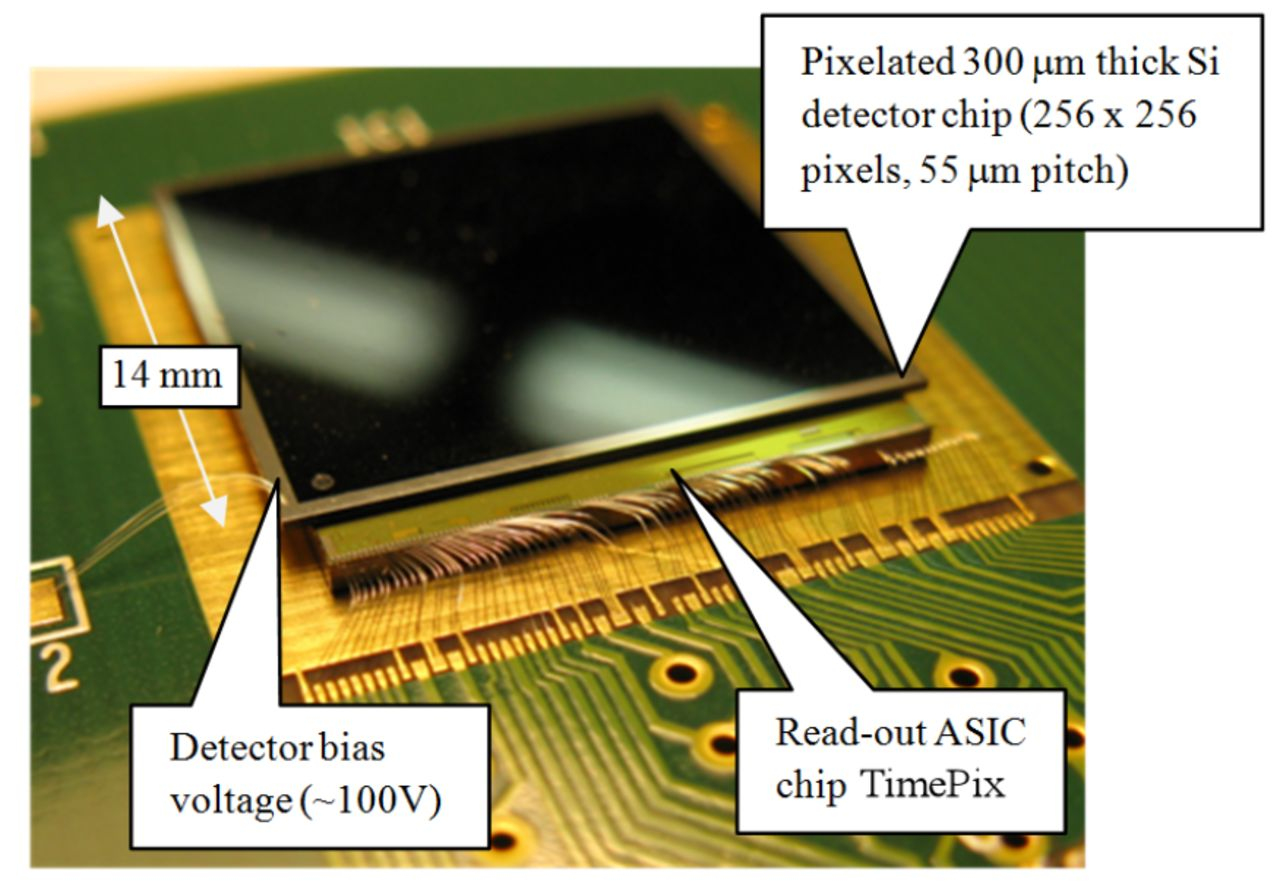
\includegraphics[width=1.0\textwidth]{./fig/timepix.jpg}
  \end{block} 
  
  \column{0.48\textwidth} % Right column and width
  \begin{block}{Timepix}
    \begin{itemize}
      \item 256$\times$256 px resolution
      \item frame-based acquisition
      \item event counting mode
      \item energy measurement mode
    \end{itemize}
  \end{block}

  \begin{block}{Timepix3}
    \begin{itemize}
      \item 256$\times$256 px resolution
      \item event-based acquisition
      \item event \& energy simultaneously
    \end{itemize}
  \end{block}

  \end{columns}

\end{frame}

\begin{frame}
\frametitle{Timepix - ...}

\begin{columns}[c]

\column{0.48\textwidth} % Right column and width

\begin{itemize}
  \item recording of the interaction of an incoming particle and the sensor
\end{itemize}

\begin{block}{Example in Figure}
\begin{enumerate}[label=(\alph*)]
  \item photons (gamma)
  \item electrons (beta)
  \item Helium nuclei (alpha)
  \item protons (heavy ions)
\end{enumerate}
\end{block}

\column{0.48\textwidth} % Left column and width
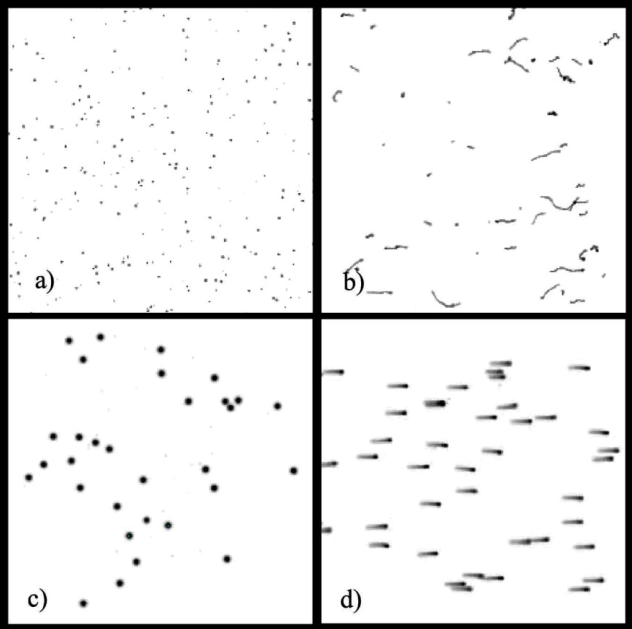
\includegraphics[width=1.0\textwidth]{./fig/particle_types_inverted.png}

\end{columns}

\end{frame}

\begin{frame}
\frametitle{VZLUSAT-1}

\fullciteinbox{baca2018timepix}{}

\end{frame}

\begin{frame}
\frametitle{Ionizing radiation dosimetry and imaging}

\fullciteinbox{baca2019timepix}{}
\fullciteinbox{stibinger2020localization}{}

\end{frame}

%%}

%%{ Publication graph

\begin{frame}
\frametitle{Research streams}

\begin{columns}[c]

\column{0.48\textwidth} % Left column and width

\centering

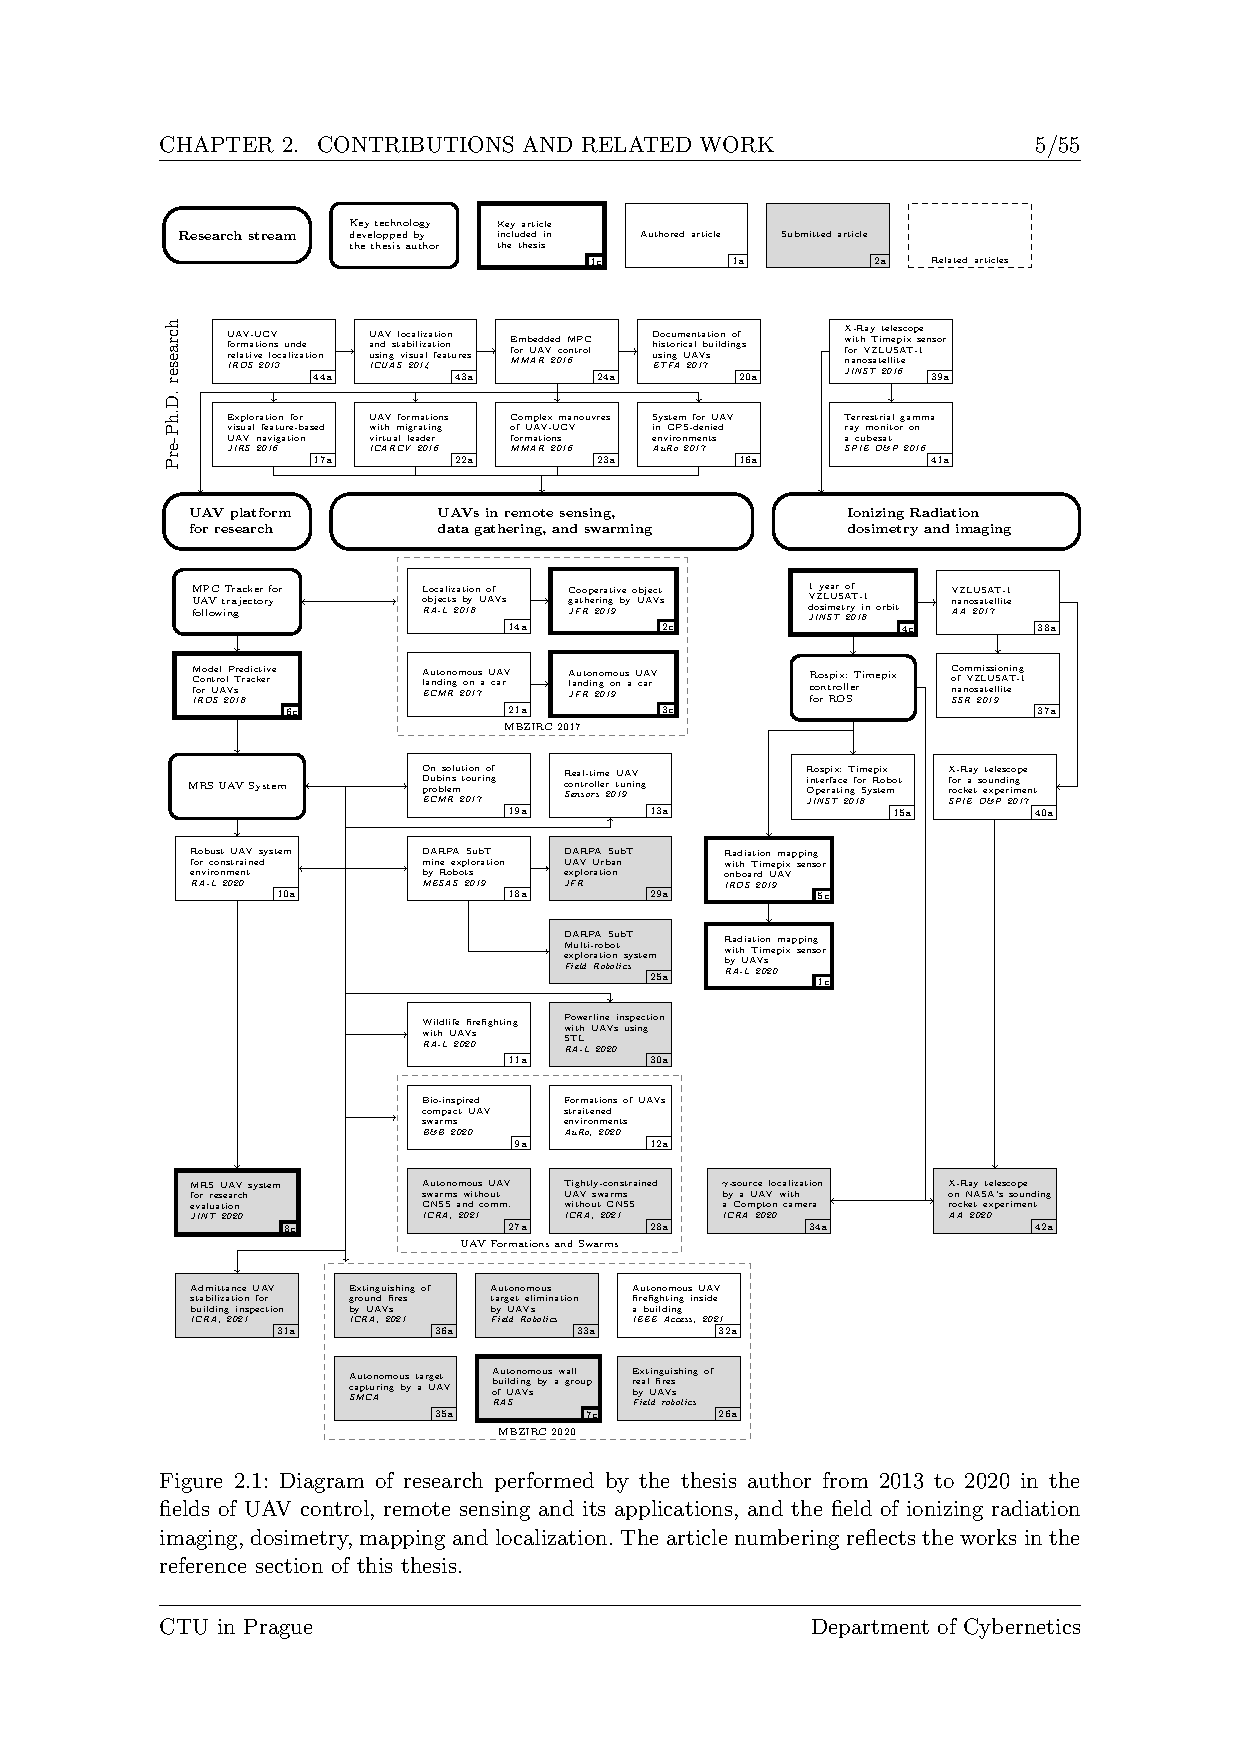
\includegraphics[width=0.9\textwidth,trim={2.0cm 5.0cm 2.5cm 5.2cm},clip]{./fig/pubgraph_january.pdf}

\centering

\column{0.48\textwidth} % Right column and width

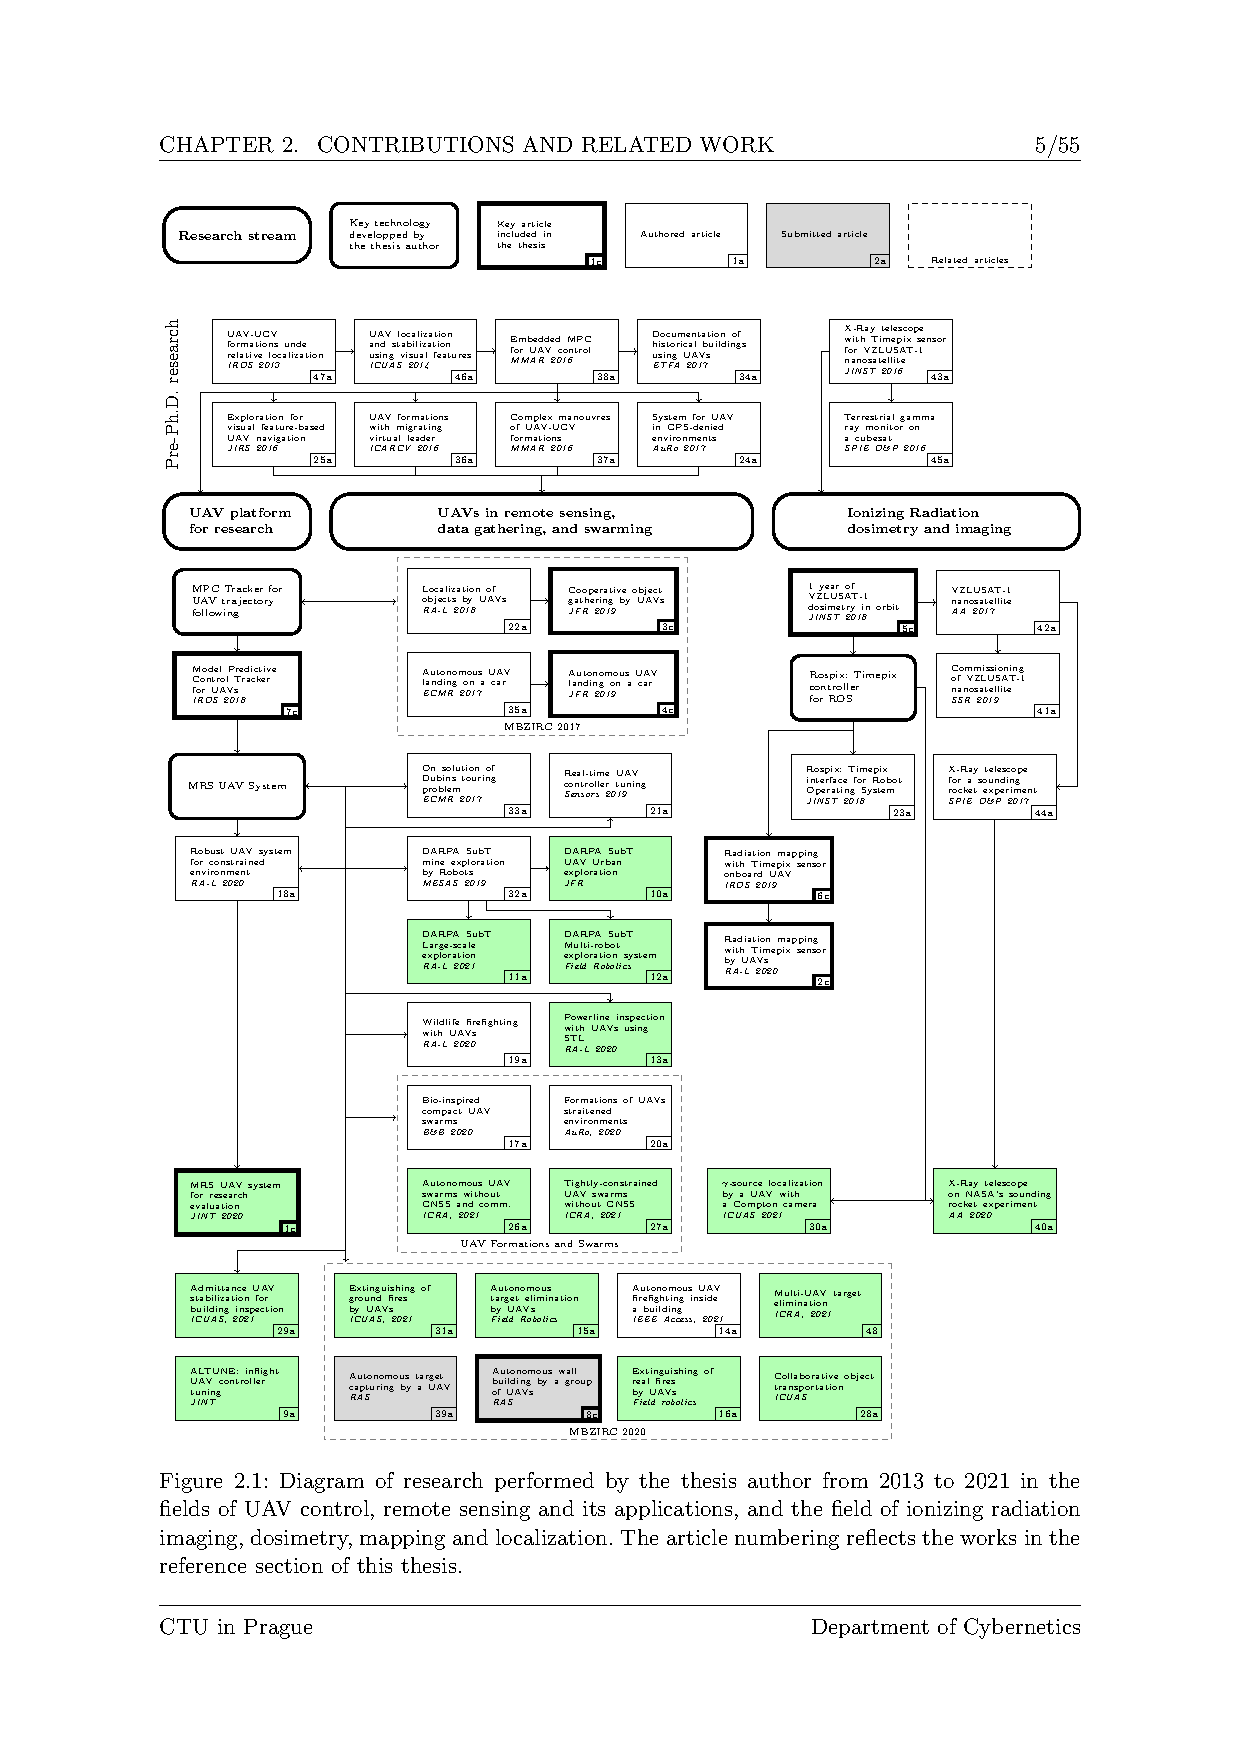
\includegraphics[width=0.9\textwidth,trim={2.0cm 5.0cm 2.5cm 5.2cm},clip]{./fig/pubgraph.pdf}

\end{columns}

\end{frame}

%%}

\section{Discussion and results}

%%{ Discussion 

\begin{frame}
\frametitle{Discussion and results}



\end{frame}

%%}

%%{ Conclusion

\begin{frame}
  \frametitle{Conclusion}

  \begin{center}
    \huge Thanks for your attention\\
    \vspace{1em}
    \large \url{http://mrs.felk.cvut.cz/people/tomas-baca}
  \end{center}

\end{frame}

%%}

%%{ References

\DeclareCiteCommand{\fullcite}
{\usebibmacro{prenote}}
{\clearfield{addendum}%
  \usedriver
  {\defcounter{minnames}{6}%
  \defcounter{maxnames}{6}}
{\thefield{entrytype}}}
{\multicitedelim}
{\usebibmacro{postnote}}

\begin{frame}
  \frametitle{Core publications}
  \tiny{
    \printbibliography[keyword={mine},keyword={phd_related},keyword={core},heading=none,title={}]
  }
\end{frame}

\begin{frame}[allowframebreaks]
  \frametitle{Other authored publications}
  \tiny{
    \printbibliography[keyword={mine},notkeyword={core},heading=none,title={}]
  }
\end{frame}

%%}

%% | ---------------------- BACKUP SLIDES --------------------- |

%%{ Research visits and stays

\begin{frame}[noframenumbering]
\frametitle{Research visits and stays abroad}

  \begin{itemize}
    \item 2015 University of Iowa, USA, 2 weeks, \emph{X-Ray testing of VZLUSAT-1 payload}
    \item 2016 University of Pennsylvania, USA, 2 months, \emph{kick-off for MBZIRC 2017}
    \item 2017 United Arab Emirates, 3 weeks, \emph{MBZIRC 2017}
    \item 2017 Pennsylvania state Univ., USA, 2 weeks, \emph{REX X-Ray testing}
    \item 2018 University of Pennsylvania, USA, 1 month, \emph{kick-off for MBZIRC 2020}
    \item 2018 Pennsylvania state Univ., USA, 2 weeks, \emph{REX assembly}
    \item 2019 Colorado, USA, 2 weeks, \emph{DARPA SubT STIX}
    \item 2019 Pennsylvania state Univ., USA, 1 week, \emph{REX dissassembly}
    \item 2020 United Arab Emirates, 5 weeks, \emph{MBZIRC 2020}
    \item 2021 United Arab Emirates, 1 month, \emph{TII collaboration}
    \item 2021 Kentucky, USA, 3 weeks, \emph{DARPA SubT Finals}
  \end{itemize}

\end{frame}

%%}

\end{document}
